%% SW arkitektur: Deployment View

Deployment view skal illustrere hvor hvilke lag af software ligger på vores platforme. Devkit8000 kører Linux og har derfor flere softwarelag end PSoC'en.
 
\vspace{15 mm}

\begin{figure}[htbp] \centering
{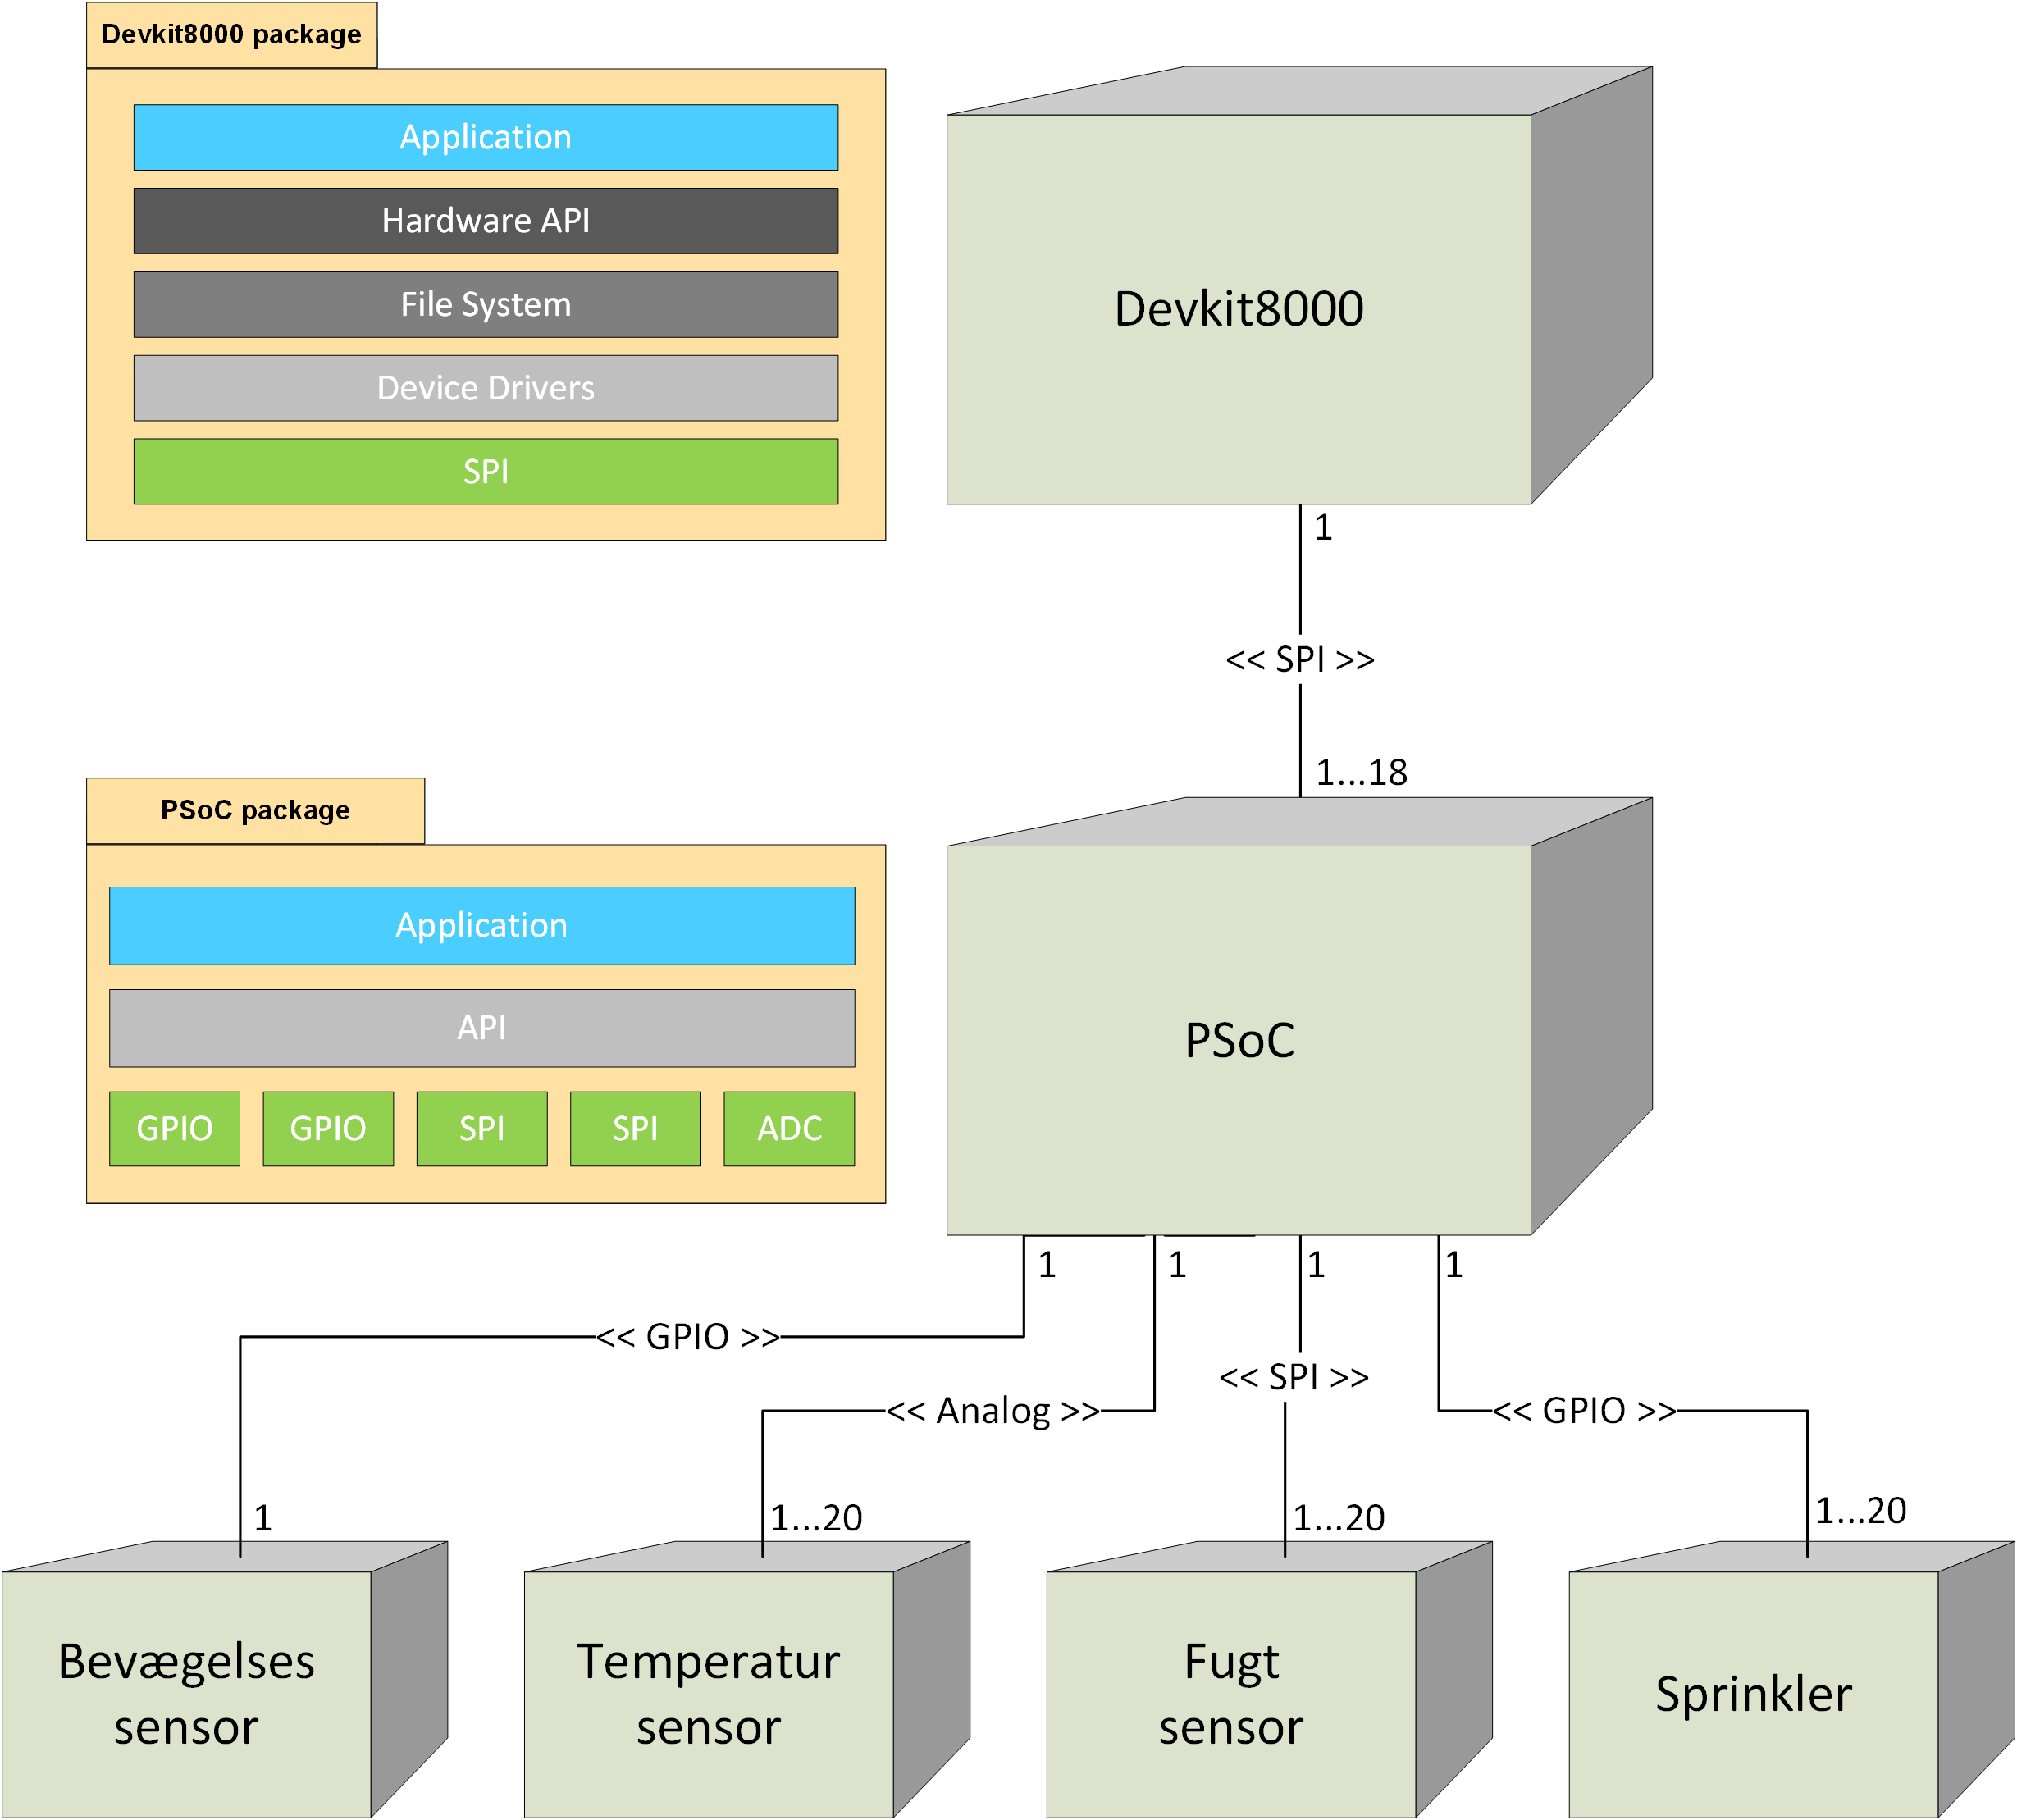
\includegraphics[scale=0.7]{filer/systemarkitektur/Deployment_model}}
\caption{Deployment model illustrerer de forskellige software og hardware(grønne) lag}
\label{fig:Deployment Model}
\end{figure}

<<<<<<< HEAD
=======
\vspace{5 mm}

\subsubsection{Devkit8000}
\textit{Applications} laget består af al den software som har med brugeren at gøre, dvs. UI og tilhørende controllers. Applicationslaget tager imod input fra brugeren og reagerer på det enten ved at kalde nogle af sine egne controllers eller sende kommandoer til hardware APIen. Laget skal desuden få data fra nedenstående lag til at fremstå overskueligt over for brugeren.

>>>>>>> origin/master
\clearpage

\begin{figure}[!htbp] \centering
{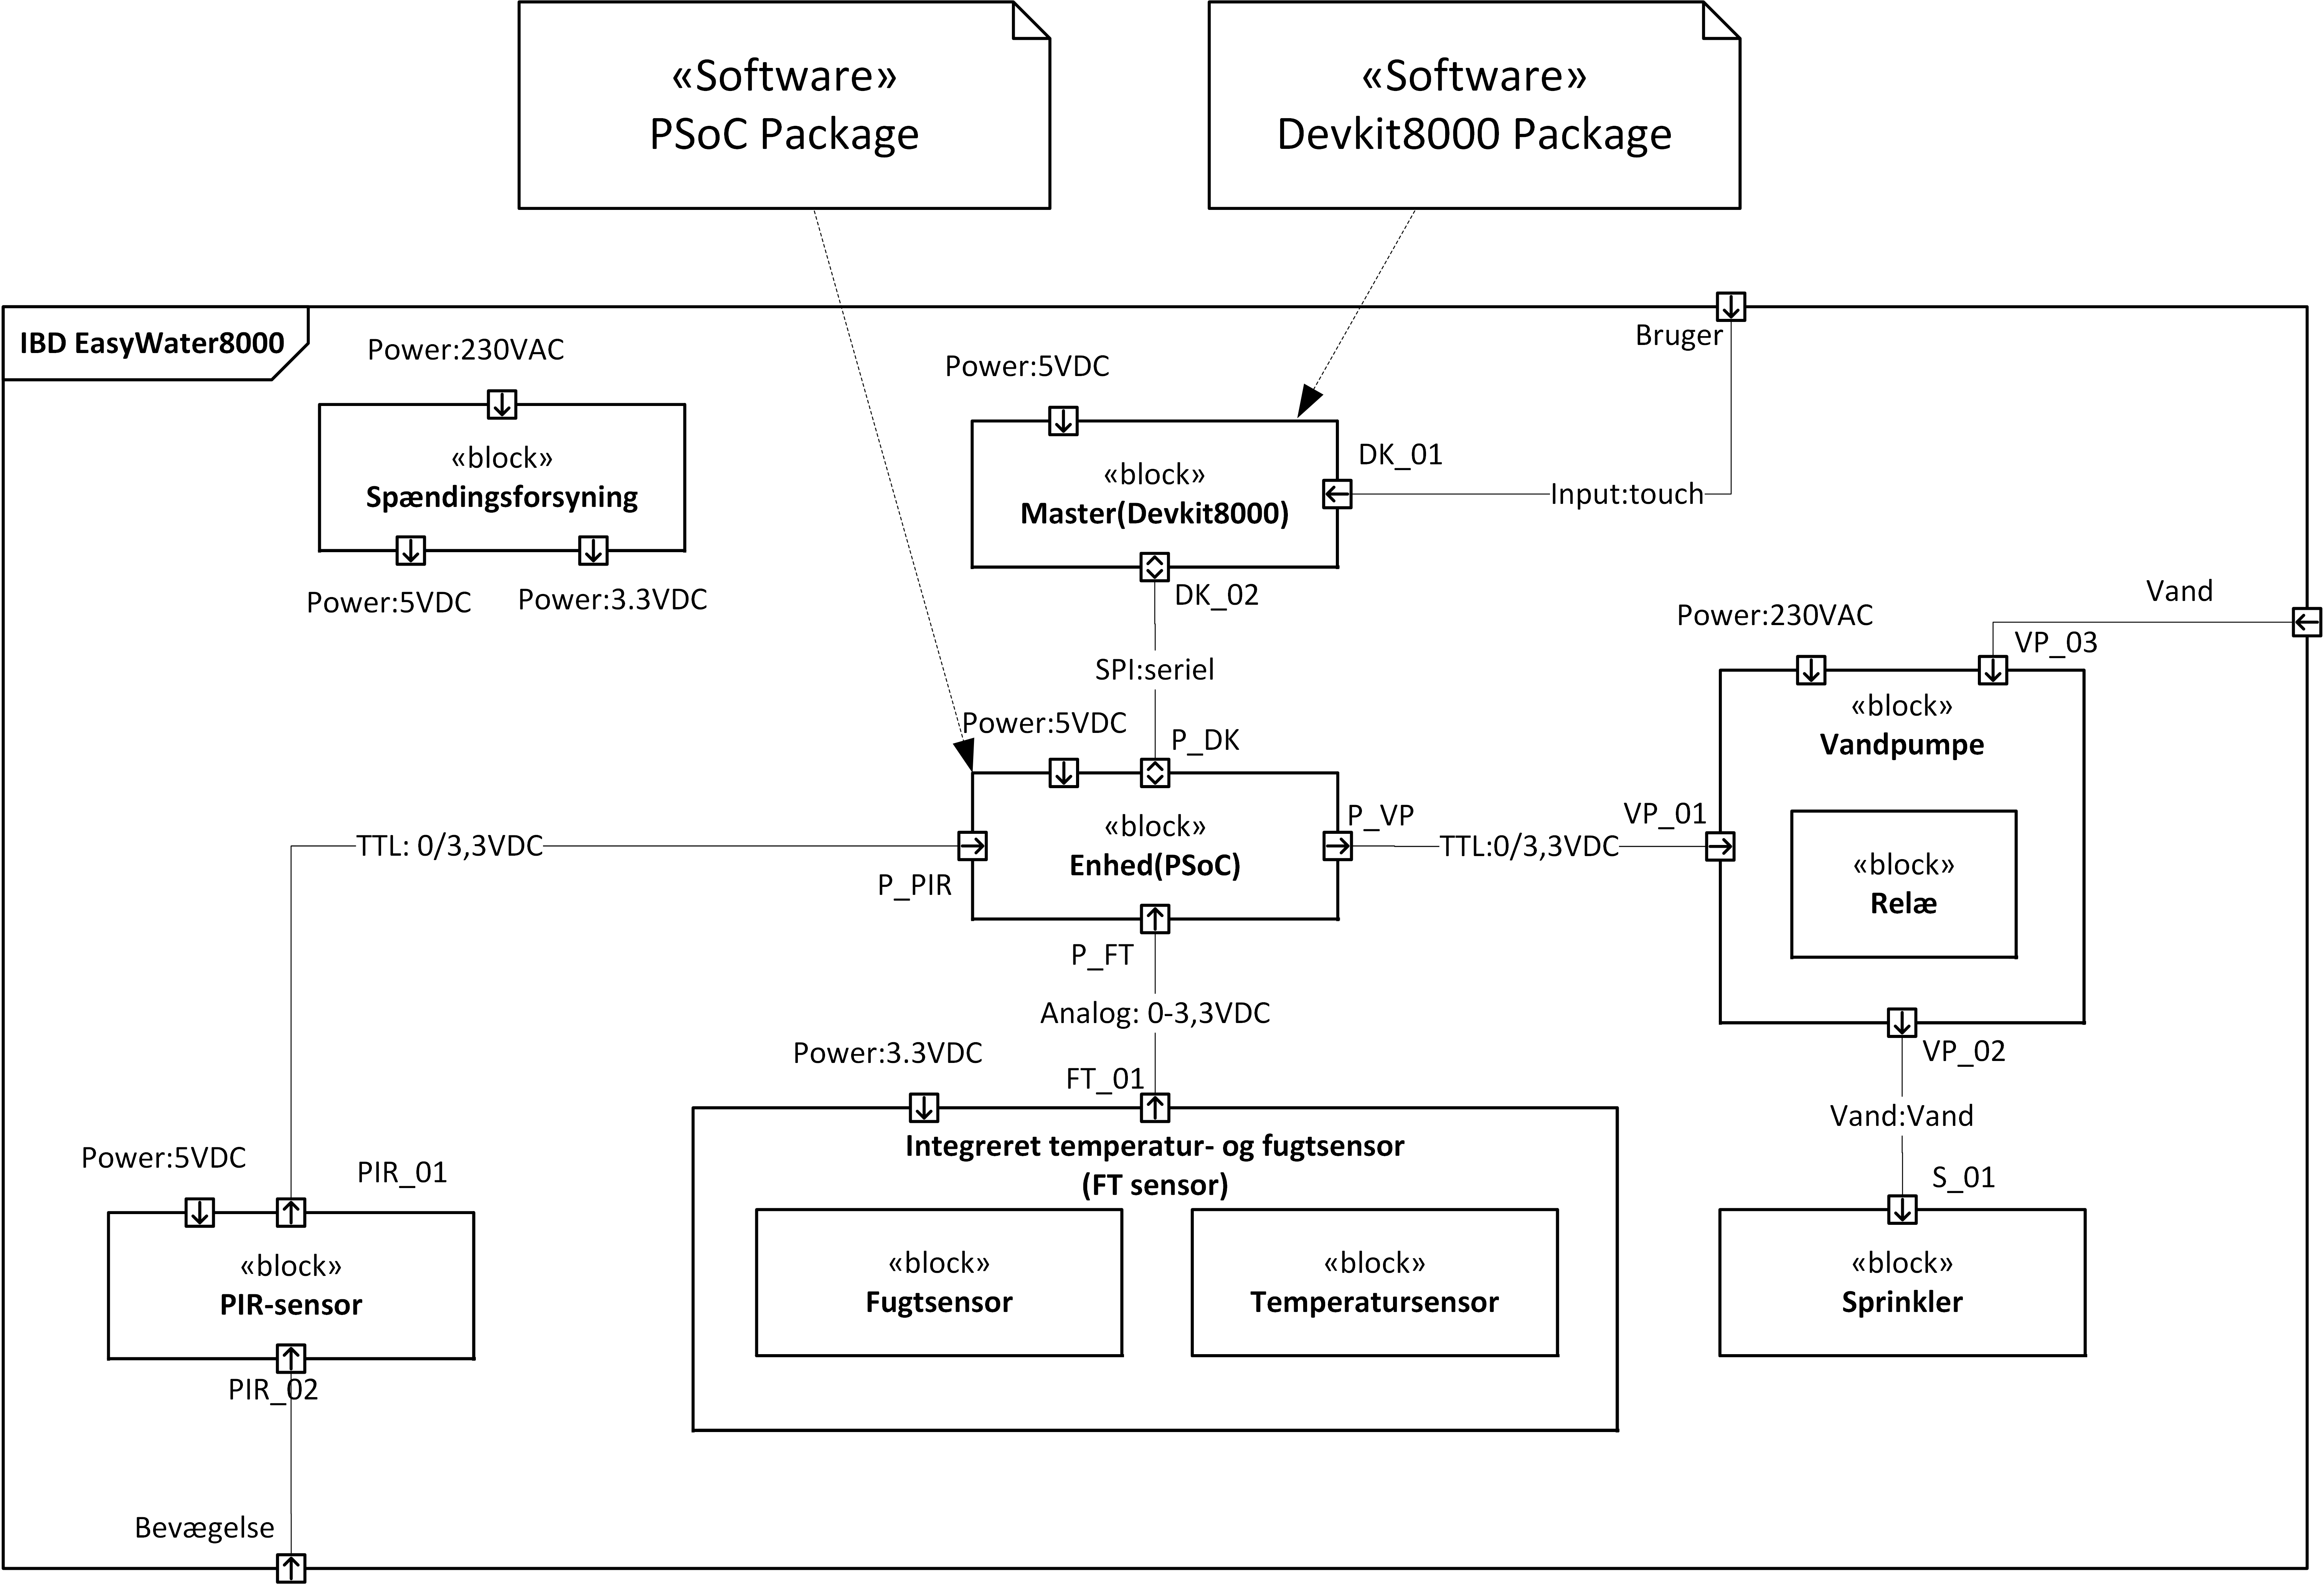
\includegraphics[scale=0.7]{filer/systemarkitektur/IBD_deployment}}
\caption{IBD med software packages}
\label{fig:IBD deployment}
\end{figure}

